% Copyright 2023 Kieran W Harvie. All rights reserved.

\section{Parabola}
For a while I've wanted to know more about conic sections and have decided that the parabola is a good plaything to start with.

\subsection{Analytic versus Synthetic}
The analytic-synthetic distinction exists in multiple fields.
Analysis means breaking something down into parts while synthesis builds something up.

A classic example is analytic-synthetic truths from Kant.
An analytic truth is ones whose truth comes from being broken down to definitions, "A number is even or it is odd" and "All bachelors are unmarried".
A synthetic truth is one whose truth depends on the real world (or is "built" from it), "The sky is blue".
\\

Like with all philosophy many will argue over my choice of examples,
but in geometry the divide is less likely to start an argument.
An analytic geometric argument breaks the figure down to coordinates while a synthetic one builds new figures up.
\\

To demonstrate the difference I will present two argument for the same result:
"Let a point $P$ be on a parabola with focus $F$.
Drop a line $PT$ such that it is perpendicular to, and $T$ is on, the directrix.
Then the tangent going though $P$ is the perpendicular bisector of $FT$."

\begin{center}
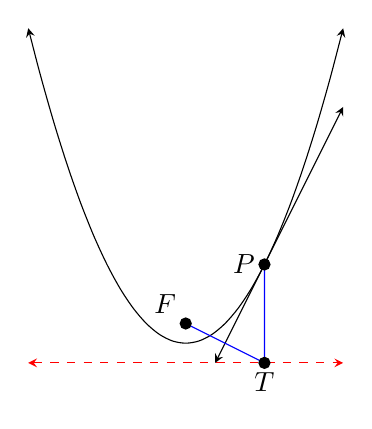
\begin{tikzpicture}[every node/.style={black}]
\draw[stealth-stealth] plot[smooth,domain=-2:2] (\x, {\x*\x});
\draw[stealth-stealth, dashed, red] (-2,-0.25) -- (2,-0.25);
\draw[stealth-stealth] (0.375,-0.25) -- (2,3);

\draw[blue] (1,1)--(1,-0.25) -- (0,0.25);

\filldraw (1,1) node[left] {$P$} circle (2pt);
\filldraw (1,-0.25) node[below] {$T$} circle (2pt);
\filldraw (0,0.25) node[above left] {$F$} circle (2pt);
\end{tikzpicture}
\end{center}

\subsubsection{Synthetic}
\begin{center}
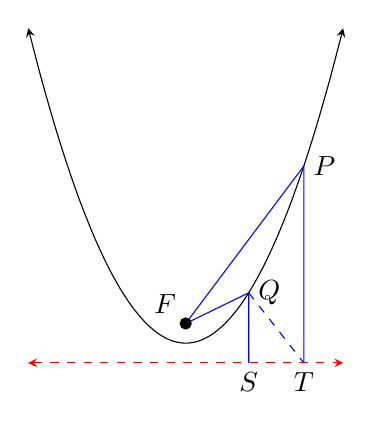
\begin{tikzpicture}[every node/.style={black}]
\draw[stealth-stealth] plot[smooth,domain=-2:2] (\x, {\x*\x});
\draw[stealth-stealth, dashed, red] (-2,-0.25) -- (2,-0.25);

\draw[blue] (0,0.25) -- (1.5,2.25) node[right] {$P$} -- (1.5,-0.25) node[below, black] {$T$};
\draw[blue] (0,0.25) -- (0.8,0.64) node[right] {$Q$} -- (0.8,-0.25) node[below, black] {$S$};
\draw[blue, dashed] (0.8,0.64) -- (1.5,-0.25);

\filldraw (0,0.25) node[above left] {$F$} circle (2pt);
\end{tikzpicture}
\end{center}
Let $F$ be the focus of the parabola,
let $P$ and $Q$ be distinct points on the parabola,
and let $T$ and $S$ be points of the directrix such that $PT$ and $QS$ are perpendicular to the directrix.
\\

By definition of a parabola $|QF|=|QS|$ and $|PF|=|PT|$,
and by construction $\triangle QST$ is a right angled triangle,
meaning:
\begin{equation*}
\begin{aligned}
|QT|^2 =& |QS|^2+|ST|^2 \\
=& |QF|^2+|ST|^2 \\
\Rightarrow |QT| >& |QF| \\
\end{aligned}
\end{equation*}

Hence the general point $Q$ isn't on the perpendicular bisector of $FT$,
but $P$ is, 
hence the perpendicular bisector of $FT$ is the tangent at $P$.

\subsubsection{Analytical}
Without loss of generality consider the unit parabola given by:
\[u: y=x^2\]
I state, without proof, that the focus is at $F=\left(0,\frac{1}{4}\right)$ and the directrix is given by:
\[d: y = -\frac{1}{4}\]
The tangent of $u$ at $P=(p,p^2)$ is given by:
\[t: y = 2px-p^2\]
Let $T=\left(p,-\frac{1}{4}\right)$ be the point of directrix such that $PT$ is perpendicular to it.
The line connecting the focus to $T$ is given by:
\[a: y= -\frac{x}{2p}+\frac{1}{4}\]
$a$ and $t$ are perpendicular since the product of their gradients is $-1$:
\[-\frac{1}{2p}\times 2p = -1\]
Also notice that the midpoint of $FT$ is given by:
\[M=\left(\frac{1}{2}(p+0),\frac{1}{2}\left(-\frac{1}{4}+\frac{1}{4}\right)\right) = \left(\frac{p}{2},0\right)\]
Is a point on both $a$ and $t$.

\subsection{Elementary Results}
\subsubsection{All points on a parabola are on the same side of the directrix as the focus:}
\begin{center}
\begin{tikzpicture}[every node/.style={black}]
	\draw[red,dashed,stealth-stealth] (-2.5,0) -- (2.5,0);
	\draw (-2,2) coordinate (F) node[above] {$F$} 
	-- (0,0) coordinate (Q) node[below] {$Q$} 
	-- (2,-2) coordinate (P) node[below] {$P$} 
	-- (2,0) coordinate (T) node[above] {$T$}
	pic[draw] {right angle = Q--T--P};
\end{tikzpicture}
\end{center}
Let $P$ be a point on the parabola on the opposite side of the focus $F$.
Let $T$ be a point on the directrix such that $PT$ is perpendicular to it.
Since $P$ and $F$ are on opposite sides of the directrix there is a point $Q$ where the segment $FP$ intersects the directrix.
\[|FP| > |QP| > |TP|\]
Which contradicts $|FP|=|TP|$,
hence $P$ doesn't exist.

\subsubsection{A line perpendicular to the directrix intersects a parabola at most once:}
\begin{center}
\begin{tikzpicture}[every node/.style={black}]
	\draw[red,dashed,stealth-stealth] (-2.5,0) -- (2.5,0);
	\coordinate (F) at (-1,3);
	\coordinate (P) at (1,4);
	\coordinate (Q) at (1,2);
	\coordinate (T) at (1,0);
	\coordinate (O) at (0,0);

	\draw (F) node[left] {$F$}
	-- (P) node[right] {$P$}
	-- (T) node[below] {$T$};

	\draw (F) -- (Q) node[right] {$Q$};

	\pic[draw] {right angle = Q--T--O};
\end{tikzpicture}
\end{center}
Let $T$ be the point where a perpendicular line to the directrix intersects the directrix.
Let $P$ and $Q$ be points on the same perpendicular line.
From the previous results both $P$ and $Q$ are on the same side as the focus $F$.
Without loss of generality let $P$ be the point further away from the directrix.
\\

Since $P$ and $Q$ are points on the parabola we have:
\[|FP| = |PT|\text{ and }|FQ| = |QT|\]
Substituting into the triangle inequality gives:
\begin{equation*}
\begin{aligned}
	|PT| =& |PQ|+|QT| \\
	=& |PQ| + |QF| \\
	>& |PF| \\
\end{aligned}
\end{equation*}
Which contradicts $|FP|=|TP|$,
hence distinct $P$ and $Q$ don't exist.

\subsubsection{A line perpendicular to the directrix intersects a parabola at least once:}
\begin{center}
\begin{tikzpicture}[every node/.style={black}]
	\draw[red,dashed,stealth-stealth] (-4.5,0) -- (2.5,0);
	\coordinate (F) at (-1,2);
	\coordinate (P) at (1,4);
	\coordinate (T) at (1,0);

	\draw (F) node[left] {$F$}
	-- (P) node[right] {$P$}
	-- (T) node[below] {$T$}
	-- (F);

	\pic[draw] {right angle = T--F--P};
\end{tikzpicture}
\end{center}
Let $F$ be the focus and let $T$ be a point on the directrix.
Extend a perpendicular line out from $T$, 
if the perpendicular intersects $F$ then the midpoint $M$ of $FT$ is on the parabola since:
\[|MF| = |MT|\]

If the perpendicular line doesn't go through $F$ suspend a second perpendicular line from the first perpendicular line at $F$ and let the two lines intersect at the point $P$.
\\

Let $X$ be a point on the segment $PT$ and define the function:
\[f(X) = |XF|-|XT|\]
We have:
\[f(T) = |TF|-|TT| > 0\]
and since $\angle PFT$ is a right angle we have $|PF| < |PT|$:
\[f(P) = |PF|-|PT| < |PT| -|PT| = 0\]
Hence by continuity there is a point $X_0$ in the segment $PT$ such that:
\[f(X_0) = 0\]
Meaning:
\[|X_0F| = |X_0T|\]
As required.

\subsubsection{A line perpendicular to the directrix intersects a parabola exactly once:}
Combine the last two results.

\subsubsection{Remarks}
These arguments are non-euclidean in two senses.
Neither sense as cool as "non-euclidean" sounds,
both of them still interesting.
\\

Firstly, is the use of continuity in the penultimate result.
The euclidean axioms famously don't include a concept of continuity.
Adding a continuity axiom to Euclid and when the concept is implicitly used has been an ongoing topic of research since the 19th century.
\\

Secondly, is the reverse.
Instead of using an another one,
we might not need to use all the euclidean axioms.
The first results don't use right-angles beyond showing $|PQ| > |PT|$ and the second result doesn't use them at all.
To me, this suggests that these results can be generalized to some subset of euclidean geometry.
I wasn't able to do so here,
but thoughts like this are why I wanted to think about parabolas more.

%% An unused diagram I don't feel like deleting.
%
%\begin{center}
%\begin{tikzpicture}[every node/.style={black}]
%	\coordinate (F) at (-2,0);
%	\coordinate (P) at (0,2);
%	\coordinate (Q) at (0,-2);
%	\coordinate (T) at (2,0);
%
%	\draw (F) node[left] {$F$} 
%	-- (P) node[above] {$P$}
%	-- (T) node[right] {$T$}
%	-- (Q) node[below] {$Q$}
%	-- (F);
%
%	\draw[red,dashed] (P) -- (Q);
%\end{tikzpicture}
%\end{center}
%With $P$ and $Q$ distinct points such that:
%\[|PT| = |PF| \text{ and } |QT| = |QF|\]
%This follows from the substitution into the triangle inequality:
%\[|PT| < |PQ|+|QT|\]
%Giving:
%\[|PT| < |PQ|+|QF|\]

%% An unused parts of an argument attempting to avoid right angles in the first result
%
%Let $F$ be the focus $P$ be the point $Q$ the intersection and $T$ the minimizing point on the directrix.
%
% Assume $|FQ| > |QT|$ then:
%\[|FP| \geq  |FQ|+|QP| > |QT|+|QP| > |TP|\]
%
%We also have:
%\[|FT|+|TP| > |FP| \geq |FQ|+|QP| = |TQ|+|QP| \geq |TP| \]
